In the parametric analysis of \Cyder performance, it was shown that the 
solubility sensitivity behavior closely matched that of the \gls{GDSM} 
sensitivity behaviors. Specifically, in Figure \ref{fig:sol_result}, a sharp turnover 
is seen where the solubility limit exceeds the point at which it limits 
movement. For increased solubility limits, release remains constant.

\begin{figure}[htbp!]
\begin{center}
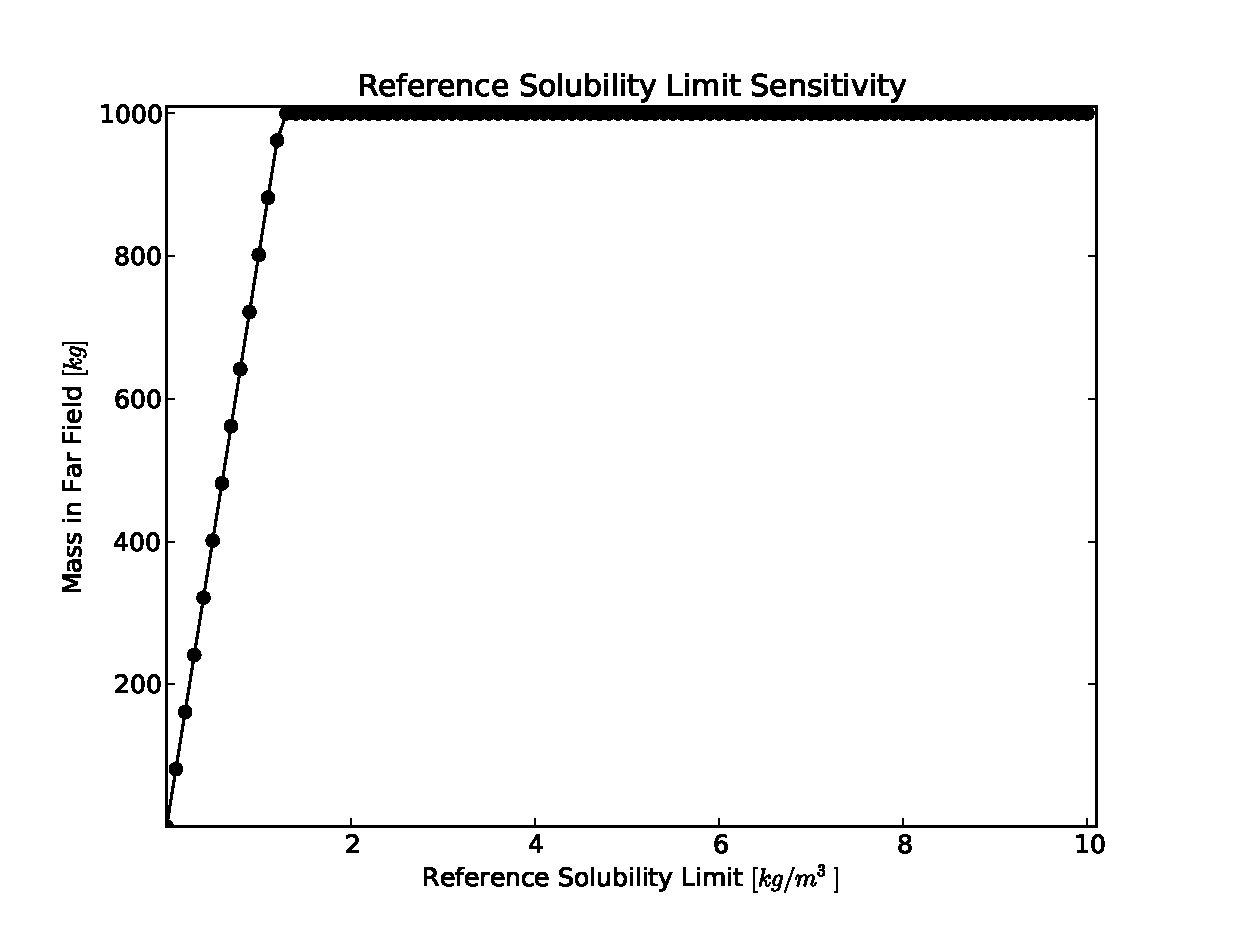
\includegraphics[width=0.7\linewidth]{./sol.eps}
\end{center}
\caption[Solubility Sensitivity in the Mixed Cell Model]{Sensitivity demonstration of solubility limitation in \Cyder for an 
arbitrary isotope assigned a variable solubility limit. }
\label{fig:sol_result}
\end{figure}

This example was conducted to show that, for an arbitrary isotope, the expected 
behavior is captured. In the case of real isotopes in a full simulation, the 
same model will be invoked with real parameters for each isotope. Thus, the 
this model agreement is representative in all cases.

